\documentclass[12pt, a4paper]{article}

% ── Packages ──────────────────────────────────────────────────
\usepackage[a4paper, top=2cm, bottom=2cm, left=1.5cm, right=1.5cm, headheight=5pt]{geometry}
\usepackage{fontenc}
\usepackage{inputenc}
\usepackage{microtype}
\usepackage{xcolor}
\usepackage{titlesec}
\usepackage{titling}
\usepackage{enumitem}
\usepackage{booktabs}
\usepackage{array}
\usepackage{tabularx}
\usepackage{fancyhdr}
\usepackage{graphicx}
\usepackage{hyperref}
\usepackage{parskip}
\usepackage{mdframed}
\usepackage{tcolorbox}
\usepackage{amsmath}
\usepackage{multirow}
\usepackage{colortbl}
\usepackage{subcaption}
% ── Colours ───────────────────────────────────────────────────
\definecolor{navy}{HTML}{0D1B2A}
\definecolor{teal}{HTML}{00A896}
\definecolor{gold}{HTML}{F4A261}
\definecolor{slate}{HTML}{4A6FA5}
\definecolor{lightgray}{HTML}{F0F4F8}
\definecolor{mutedtext}{HTML}{5A7A8A}
\definecolor{darktext}{HTML}{1A2E3B}
\definecolor{rulecolor}{HTML}{D1D5DB}

% ── Hyperref setup ────────────────────────────────────────────
\hypersetup{
  colorlinks=true,
  linkcolor=teal,
  urlcolor=teal,
  citecolor=slate,
  pdftitle={Used Car Value Tier Prediction - Data Science Project Proposal},
  pdfauthor={Project Team}
}

% ── Header / Footer ───────────────────────────────────────────
\pagestyle{fancy}
\fancyhf{}
\fancyhead[L]{\small\color{mutedtext}Used Car Value Tier Prediction}
\fancyhead[R]{\small\color{mutedtext}Data Science Project Proposal}
\fancyfoot[C]{\small\color{mutedtext}\thepage}
\renewcommand{\headrulewidth}{0.4pt}
\renewcommand{\headrule}{\hbox to\headwidth{\color{rulecolor}\leaders\hrule height \headrulewidth\hfill}}

% ── Section styling ───────────────────────────────────────────
\titleformat{\section}
  {\color{navy}\normalsize\bfseries}
  {\color{teal}\thesection}{0.3em}{}
  [\vspace{-0.4em}\color{rulecolor}\rule{\linewidth}{0.4pt}]

\titleformat{\subsection}
  {\color{darktext}\small\bfseries}
  {\color{slate}\thesubsection}{0.4em}{}

\titleformat{\subsubsection}
  {\color{mutedtext}\small\itshape}
  {}{0em}{}

\titlespacing{\section}{0pt}{0.35em}{0.05em}
\titlespacing{\subsection}{0pt}{0.25em}{0.05em}
\titlespacing{\subsubsection}{0pt}{0.2em}{0em}

% ── tcolorbox styles ──────────────────────────────────────────
\tcbuselibrary{skins, breakable}

\newtcolorbox{databox}[2]{
  enhanced,
  colback=#2!8!white,
  colframe=#2,
  boxrule=0.7pt,
  left=4pt, right=4pt, top=3pt, bottom=3pt,
  arc=4pt,
  title={\small\bfseries\color{white} #1},
  attach boxed title to top left={yshift=-2mm, xshift=6mm},
  boxed title style={colback=#2, colframe=#2, arc=3pt}
}

% ── List styling ──────────────────────────────────────────────
\setlist[itemize]{
  leftmargin=1.4em, topsep=3pt, itemsep=2pt, parsep=0pt,
  label={\color{teal}\textbullet}
}
\setlist[enumerate]{
  leftmargin=1.6em, topsep=3pt, itemsep=2pt, parsep=0pt,
  label={\color{navy}\bfseries\arabic*.}
}

\title{}
\date{}

% ══════════════════════════════════════════════════════════════
\begin{document}
\thispagestyle{empty}

% ── Cover page ────────────────────────────────────────────────
\begin{center}
\begin{center}

    % --- Header Logos ---
    \begin{minipage}[c]{0.12\textwidth}
        
\includegraphics[width=\textwidth]{Cairo_University_Crest.png}
    \end{minipage}
    \hfill
    \begin{minipage}[c]{0.6\textwidth}
        \centering
        {\large Cairo University - Faculty Of Engineering \\ 
        Computer Engineering Department \\ 
        CMP4007 Applied Data Science - Spring 2026 \par}
    \end{minipage}
    \hfill
    \begin{minipage}[c]{0.15\textwidth}
        
\includegraphics[width=\textwidth]{CUFE.jpeg}
    \end{minipage}

\end{center}

\vspace{0.5cm}
\noindent\hrulefill

\vspace{2.5cm}

  {\color{navy}\Huge\bfseries Project Proposal}\\[1.5em]
  {\color{darktext}\Large Team 9}\\[0.5em]
  {\color{mutedtext}Eng. Eman Hosam}\\
\end{center}
\vspace{2.5cm}

% ── Team Table ────────────────────────────────────────────────
\begin{center}
\renewcommand{\arraystretch}{1.6}
\begin{tabular}{c l c c c}
  \rowcolor{navy}
  {\color{white}\small\bfseries \#} &
  {\color{white}\small\bfseries Name} &
  {\color{white}\small\bfseries ID} &
  {\color{white}\small\bfseries Section} &
  {\color{white}\small\bfseries Bench No.} \\
  \rowcolor{lightgray}
  1 & Ahmed Hamdy & 9220032 & 1 & 4 \\
  \rowcolor{white}
  2 & Ahmed Aladdin & 9220065 & 1 & 5 \\
  \rowcolor{lightgray}
  3 & Asmaa Mohamed & 9220154 & 1 & 29 \\
  \rowcolor{white}
  4 & Shehab Khaled & 9220393 & 1 & 38 \\
\end{tabular}
\end{center}


\newpage
\tableofcontents
\newpage
\section{Problem Definition \& Business Context}

\subsection{Business Problem}
Used car dealerships and online marketplaces receive large volumes of vehicle listings and trade-ins. Manually assigning each vehicle into a pricing/value tier is time-consuming and inconsistent across staff and branches. This project aims to automate the classification of incoming used cars into value tiers using historical market data.

\subsection{Stakeholder}

\begin{itemize}
  \item Primary: Used Car Dealerships (pricing and inventory teams)
  \item Secondary: Online Marketplaces (listing recommendations) and Insurance Underwriters (risk and valuation support)
\end{itemize}

\subsection{Problem Formulation}

This problem is formulated as a \textbf{classification task}, where the goal is to predict the \textbf{price/value tier} of a used car listing.

\textbf{Tier Definition:} Cars are grouped into \textbf{Budget}, \textbf{Mid-Range}, and \textbf{Luxury} tiers based on price.
\subsection{Justification for Classification}

\begin{itemize}
  \item The target is a discrete set of tiers (Budget / Mid-Range / Luxury)
  \item Tier outputs support operational decisions (pricing, procurement, and marketing)
  \item Classification enables threshold-based policies and consistent segmentation
\end{itemize}

\subsection{Business Impact}

\begin{itemize}
  \item Faster and more consistent inventory categorization
  \item Improved pricing strategy and margin optimization
  \item Better customer targeting (budget buyers vs. premium buyers)
\end{itemize}

% ══════════════════════════════════════════════════════════════
\section{Datasets}

\subsection{Primary Source (Kaggle Dataset)}
\textbf{Source:} Kaggle --- \emph{Uncovering Factors That Affect Used Car Prices} \\
\textbf{URL:} \href{uncovering-factors-that-affect-used-car-prices}{https://www.kaggle.com/datasets/thedevastator/uncovering-factors-that-affect-used-car-prices}
% \url{https://www.kaggle.com/datasets/thedevastator/uncovering-factors-that-affect-used-car-prices}

\begin{databox}{autos.csv}{teal}
  Main structured dataset (CSV). Each row represents a used car listing with attributes such as price, brand, model, registration year, mileage, and fuel type.
\end{databox}

\subsection{Secondary Source (Web Scraping)}
\textbf{Source:} AutoScout24 \\
\textbf{URL:} \url{https://www.autoscout24.com}

\begin{databox}{AutoScout24 Listings}{slate}
  Scraped used car listings to increase coverage and validate pricing patterns.
\end{databox}
\newpage
\subsection{Feature Documentation (Core Fields)}

The main features to be used in modelling (10+ fields):
\begin{center}
\renewcommand{\arraystretch}{1.6}
\begin{tabular}{c l c c}
  \rowcolor{navy}
  {\color{white}\small\bfseries \#} &
  {\color{white}\small\bfseries Feature} &
  {\color{white}\small\bfseries Type} &
  {\color{white}\small\bfseries Description} \\
  \rowcolor{lightgray}
  1 & seller & Categorical & seller type (business/private) \\
  \rowcolor{white}
  % 2 & abtest & Categorical & Test type (A or B) \\
  % \rowcolor{lightgray}
  2 & vehicleType & Categorical & body type \\
  \rowcolor{white}
  % 4 & gearbox & Categorical & transmission type \\  \rowcolor{lightgray}
  3 & yearOfRegistration & Numeric & Year the car was registered \\
  \rowcolor{white}
  4 & gearbox & Categorical & Type of gearbox (manual or automatic) \\
  \rowcolor{lightgray}
  5 & power & Numeric & Power of the car in Horse Power \\
  \rowcolor{white}
  % 8 & model & Categorical & Model of the car \\
  % \rowcolor{lightgray}
  6 & brand & Categorical & Brand of the car \\
  \rowcolor{white}
  7 & kilometers & Numeric & Kilometers the car has been driven \\
  \rowcolor{lightgray}
  8 & fuelType & Categorical & Type of fuel (e.g. diesel, petrol, etc.) \\
  \rowcolor{white}
  % 9 & vehicleAge (Engineered) & Numeric &  Current Year - Registration Year  \\
  % \rowcolor{lightgray}
  % 10 & kmPerYear (Engineered) & Numeric & kilometers / (vehicleAge + 1) \\
  % \rowcolor{white}
  % \rowcolor{lightgray}
  % 14 & monthOfRegistration & Numeric & Month the car was registered\\ 
\end{tabular}
\end{center}
\vspace{0.25cm}
\textbf{Note:} After deriving the tier label from \texttt{price}, the raw \texttt{price} feature will not be used as an input feature to avoid target leakage 

\subsection{Engineered Features (Planned)}
In addition to the core fields, we plan to engineer the following features:
\begin{itemize}
  \item \textbf{vehicleAge} = current\_year (2026) $-$ yearOfRegistration
  \item \textbf{kmPerYear} = kilometers / (vehicleAge + 1)
  \item \textbf{isAutomatic} = (gearbox == "automatic")
  \item \textbf{is\_vintage\_classic} derived from vehicleAge \& brand
  \item \textbf{power\_to\_tier\_bin} derived from powerPS
\end{itemize}

% ══════════════════════════════════════════════════════════════
\newpage
\section{Data Acquisition \& Integration}

\subsection{Data Acquisition}

\begin{itemize}
  \item Kaggle dataset downloaded as CSV file(s) (e.g., \texttt{autos.csv}).
  \item AutoScout24 listings collected via web scraping using Python (e.g., \texttt{Scrapy} + \texttt{Scrapy-Splash}).
\end{itemize}

\subsection{Data Integration Strategy}

\begin{itemize}
  \item \textbf{Vertical merge} the Kaggle dataset with scraped AutoScout24 listings by aligning both sources to a unified schema.
  \item Standardize fields (e.g., currency, mileage units, categorical labels) and resolve naming differences (e.g., \texttt{kilometers} vs \texttt{mileage}).
  \item Deduplicate near-identical listings using matching keys such as \textbf{brand}, \textbf{model}, \textbf{yearOfRegistration}, \textbf{kilometers}, and \textbf{power}.
  \item Merge strategy:
  \begin{itemize}
    \item Union rows after schema alignment (preferred for coverage)
    \item Optional record linkage to detect overlaps across sources
  \end{itemize}
  \item Handle missing fields introduced by scraping or schema differences using imputation or "unknown" categories.
\end{itemize}

\textbf{Challenges:}
\begin{itemize}
  \item Inconsistent naming and category sets across sources
  \item Translating the Kaggle dataset from German to English
  \item Currency and locale differences
  \item Missing or noisy scraped fields due to unstructured HTML
  \item Potential duplicates across sources
\end{itemize}

% ══════════════════════════════════════════════════════════════
\section{Target Variable}

\begin{databox}{Target Definition}{gold}
PRICE\_TIER = value tier derived from listing \texttt{price}.
\end{databox}

\textbf{Tier Construction:}
\begin{center}
\renewcommand{\arraystretch}{1.6}
\begin{tabular}{c l c c c}
  \rowcolor{slate}
  {\color{white}\small\bfseries Tier} &
  {\color{white}\small\bfseries Label} &
  {\color{white}\small\bfseries Price Range} &
  {\color{white}\small\bfseries Business Meaning} &
  {\color{white}\small\bfseries Business Interpretation}\\
  \rowcolor{lightgray}
  0 & Budget & $\leq$ \$5,000 & High-mileage or older cars & Entry-level pricing segment \\
  \rowcolor{white}
  1 & Mid-Range &  \$5,000 - \$15,000 & Recent-model mid-size cars & Mainstream segment\\
  \rowcolor{lightgray}
  2 & Luxury & $>$ \$15,000 & Luxury, electric, or new cars & Premium segment\\
\end{tabular}
\end{center}
\vspace{0.25cm}


\textbf{Class Distribution} [62.90\% Budget, 25.57\% Mid-Range, 8.62\% Luxury]

\begin{figure}[htbp]
     \centering
     % First Image
     \begin{subfigure}[b]{0.50\textwidth}
         \centering
         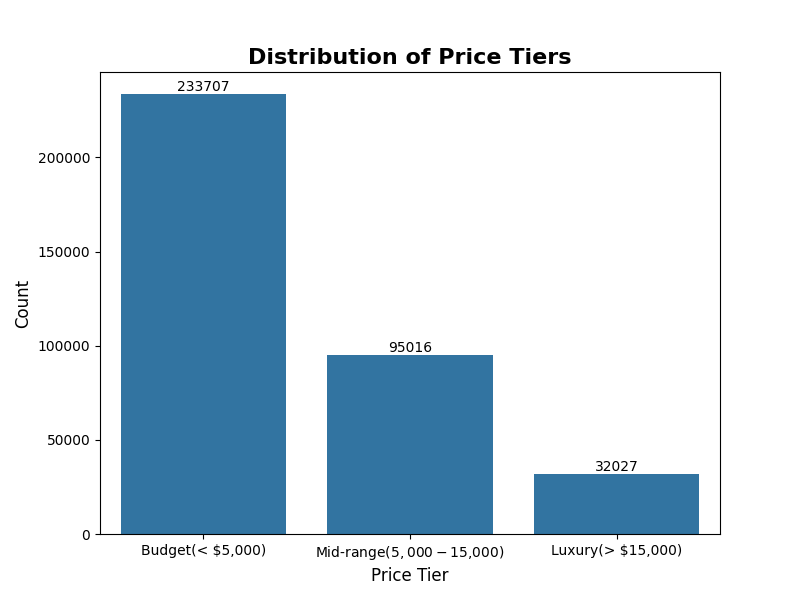
\includegraphics[width=1\textwidth]{figures/price_tier_distribution.png}
         \label{fig:image1}
     \end{subfigure}
     % Second Image
     \begin{subfigure}[b]{0.49\textwidth}
         \centering
         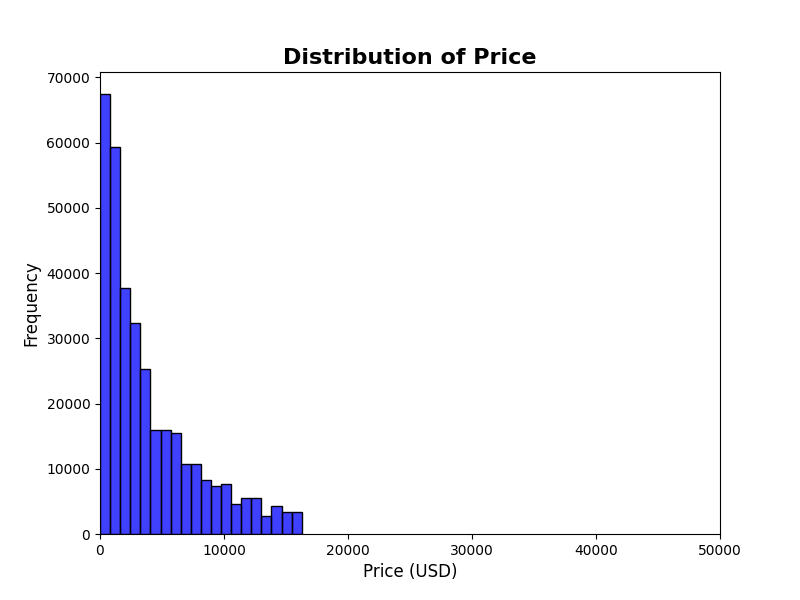
\includegraphics[width=1\textwidth]{figures/price_distribution.png}
         \label{fig:image2}
     \end{subfigure}
     
     \caption{Left: Target tier counts. Right: Raw price histogram.}
     \label{fig:target_distribution}
\end{figure}
% ══════════════════════════════════════════════════════════════
\newpage
\section{Data Validation Report}

\subsection{Dataset Overview}
\vspace{0.25cm}
\begin{center}
\renewcommand{\arraystretch}{1.6}
\begin{tabular}{c c}
  \rowcolor{slate}
  {\color{white}\small\bfseries Metric} &
  {\color{white}\small\bfseries Value} \\
  \rowcolor{lightgray} Total rows (raw)& 371528 \\
  \rowcolor{white}  Total columns & 21 \\
  \rowcolor{lightgray}  Numeric columns & 8 \\
  \rowcolor{white}  Categorical columns & 13 \\
  \rowcolor{lightgray}   Total missing cells& 194786 \\
    \rowcolor{white} Full-row duplicates& 0 \\
  \rowcolor{lightgray}   Total missing cells& 194786 \\
\end{tabular}
\end{center}
\vspace{0.25cm}
% ─────────────────────────────────────────────────────────────
\subsection{Completeness - Missing Values Analysis}
\vspace{0.25cm}
\begin{center}
\renewcommand{\arraystretch}{1.5}
\begin{tabular}{l c c c}
\rowcolor{slate}
{\color{white}\small\bfseries Column} &
{\color{white}\small\bfseries Missing Count} &
{\color{white}\small\bfseries Missing \%} &
{\color{white}\small\bfseries Status} \\

% \rowcolor{lightgray} notRepairedDamage & 72060 & 19.40\% & \textcolor{red}{WARN} \\
\rowcolor{lightgray} vehicleType & 37869 & 10.19\% & \textcolor{red}{WARN} \\
\rowcolor{white} fuelType & 33386 & 8.99\% & \textcolor{red}{WARN} \\
% \rowcolor{lightgray} model & 20484 & 5.51\% & \textcolor{red}{WARN} \\
\rowcolor{white} gearbox & 20209 & 5.44\% & \textcolor{green}{OK} \\
\rowcolor{white} price\_tier & 10778 & 2.90\% & \textcolor{green}{OK} \\
\end{tabular}
\end{center}
\vspace{0.25cm}
\newpage
% ─────────────────────────────────────────────────────────────
\subsection{Descriptive Statistics (Numeric Columns)}
\vspace{0.25cm}
\begin{center}
\renewcommand{\arraystretch}{1.4}
\begin{tabular}{l c c c c c c c c}
\rowcolor{slate}
{\color{white}\small\bfseries Column} &
{\color{white}\small\bfseries Count} &
{\color{white}\small\bfseries Mean} &
{\color{white}\small\bfseries Std} &
{\color{white}\small\bfseries Min} &
{\color{white}\small\bfseries 25\%} &
{\color{white}\small\bfseries 50\%} &
{\color{white}\small\bfseries 75\%} &
{\color{white}\small\bfseries Max} \\
\rowcolor{lightgray}
yearOfRegistration & 371528 & 2004.58 & 92.87 & 1000 & 1999 & 2003 & 2008 & 9999 \\

\rowcolor{white}
powerPS & 371528 & 115.55 & 192.14 & 0 & 70 & 105 & 150 & 20000 \\

\rowcolor{lightgray}
kilometer & 371528 & 125618.69 & 40112.34 & 5000 & 125,000 & 150,000 & 150,000 & 150,000 \\
\end{tabular}
\end{center}

\vspace{0.25cm}

% ─────────────────────────────────────────────────────────────
\subsection{Consistency - Schema \& Data Types}
\vspace{0.25cm}

\begin{center}
\renewcommand{\arraystretch}{1.4}
\begin{tabular}{l c c c}
\rowcolor{slate}
{\color{white}\small\bfseries Column} &
{\color{white}\small\bfseries Detected Type} &
{\color{white}\small\bfseries Expected Type} &
{\color{white}\small\bfseries Match} \\
\rowcolor{lightgray} dateCrawled & str & str & \textcolor{green}{Yes} \\
\rowcolor{white} model & str & object & \textcolor{green}{Yes} \\
\rowcolor{lightgray} powerPS & int64 & int64 &\textcolor{green}{Yes} \\
\rowcolor{white} kilometer & int64 & int64 & \textcolor{green}{Yes} \\
\rowcolor{lightgray} price & int64 & int64 & \textcolor{green}{Yes} \\
\rowcolor{white} name & str & str & \textcolor{green}{Yes} \\
\rowcolor{lightgray} seller & str & str &\textcolor{green}{Yes} \\
\rowcolor{white} offerType & str & str & \textcolor{green}{Yes} \\
\rowcolor{lightgray} yearOfRegistration & int64 & int64 & \textcolor{green}{Yes} \\
\rowcolor{white} gearbox & str & str & \textcolor{green}{Yes} \\
\rowcolor{lightgray} price & int64 & int64 & \textcolor{green}{Yes} \\
\rowcolor{white} vehicleType & str & str & \textcolor{green}{Yes} \\
\rowcolor{lightgray} abtest & str & str & \textcolor{green}{Yes} \\
\rowcolor{white} monthOfRegistration & str & str & \textcolor{green}{Yes} \\
\rowcolor{lightgray} fuelType & str & str & \textcolor{green}{Yes} \\
\rowcolor{white} brand & str & str & \textcolor{green}{Yes} \\
\rowcolor{lightgray} notRepairedDamage & str & str & \textcolor{green}{Yes} \\
\end{tabular}
\end{center}
\vspace{0.2cm}
All columns match expected schema with minor dtype differences are due to pandas representation.

% ─────────────────────────────────────────────────────────────
\subsection{Uniqueness - Duplicate Detection}

\begin{itemize}
  \item Full-row duplicates detected: \textbf{0 rows}
  \item Partial duplicates detected (removing dateCrawled column): \textbf{12575 rows}
\end{itemize}

% ─────────────────────────────────────────────────────────────
\subsection{Accuracy - Range \& Outlier Checks}
\vspace{0.25cm}
\begin{center}
\renewcommand{\arraystretch}{1.4}
\begin{tabular}{l c c c}
\rowcolor{slate}
{\color{white}\small\bfseries Column} &
{\color{white}\small\bfseries Rule} &
{\color{white}\small\bfseries Violation Percentage} &
{\color{white}\small\bfseries Status} \\
\rowcolor{lightgray} yearOfRegistration & [1900 - 2023] & 182 (0.05\%) & \textcolor{green}{Pass} \\
\rowcolor{white} kilometer & [0 - 300,000] & 0  & \textcolor{green}{Pass} \\
\rowcolor{lightgray} powerPS & [40 - 5,000] & 40907 (11.01\%) &\textcolor{red}{Fail} \\
\rowcolor{white} price & $>$ 0 & 0 & \textcolor{green}{Pass} \\
\end{tabular}
\end{center}
\vspace{0.25cm}
% ─────────────────────────────────────────────────────────────

\subsection{Validity - Categorical Analysis}
\textbf{Transmission Types:}
\begin{itemize}
  \item Automatic ( 73.81\%), Manual (26.19\%)
\end{itemize}

\textbf{Fuel Types:}
\begin{itemize}
  \item Benzin (60.25\%), Diesel (29.0\%), lpg (1.45\%), cng (0.15\%), Electric (0.03\%), Hybrid (0.07\%)
\end{itemize}


% ─────────────────────────────────────────────────────────────
\subsection{Distribution Checks}

\begin{center}
\renewcommand{\arraystretch}{1.4}
\begin{tabular}{l c c c c c}
\rowcolor{slate}
{\color{white}\small\bfseries Column} &
{\color{white}\small\bfseries Mean} &
{\color{white}\small\bfseries Median} &
{\color{white}\small\bfseries Std} &
{\color{white}\small\bfseries Skewness} \\
\rowcolor{lightgray} registration year & 2004.58 & 2003 & 92.87 & 72.13  \\
\rowcolor{white} price & 14716 & 14861 & 6664 & 578.06\\
\rowcolor{lightgray} kilometers & 125,618.69 & 150,000 & 40,112.34 & -1.55  \\
\rowcolor{white} powerPS & 115.55 & 105 & 192.14 & 58.2  \\
\end{tabular}
\end{center}

\vspace{0.2cm}
Distributions fall within expected business ranges after excluding invalid values.

% ─────────────────────────────────────────────────────────────
\subsection{Data Cleaning Plan}

\begin{itemize}
  \item Remove invalid rows:
  \begin{itemize}
    \item year outside [1900, 2023]
    \item kilometers outside [0, 300000]
    \item price is missing or price $<$ 100
  \end{itemize}
  \item Keep one record of the duplicated records
  \item Impute missing categorical values using mode value of the brand
  \item Standardize categorical labels across sources
\end{itemize}
\subsection{Summary of Data Quality Issues}

\begin{itemize}
  \item Missing values in key variables (vehicleType, feulType, model, gearbox, price, notRepairedDamage).
  \item Class imbalance (ratio between Budget to Luxury  $\approx$ 7.3 )
  \item Potential outliers in \texttt{power}
  \item Data integration gaps (schema differences / scraping noise)
\end{itemize}

\end{document}